\section{联邦学习数据集}
\addcontentsline{toe}{section}{{\thesection\ \ Datasets for Federated Learning}\numberline\,}
% \esection{Datasets for Federated Learning}
\label{sec:chap5-datasets}

% almost finished
% indexed

正如本报告\S\ref{sec:chap1-fl-applications}~中提到的,联邦学习所涉及、处理的实际数据往往具有强烈的统计异质性,因此用于联邦学习仿真试验的试验数据集需要以多种方式、从多个角度尽量模拟、贴近这种统计异质性。比较幸运的是,在本章\S\ref{sec:chap5-design}中提到的一些联邦学习代码框架,包括FedML\cite{he_2020_fedml}, LEAF\cite{caldas2018_leaf},以及\texttt{FedProx}\cite{sahu2018fedprox}, \texttt{IFCA}\cite{Ghosh_2022_cfl}等联邦学习算法文献,已经将多个数据集依照联邦学习场景的特点进行了相应的适配以及标准化,方便进行联邦学习算法的对比研究,以及效果复现等工作。

联邦学习仿真系统\texttt{fl-sim}将其中常用的一些联邦学习数据集封装、集成到了\texttt{data\_processing}模块中,并添加了一系列方便使用的功能,这一点已经在上一节\S\ref{sec:chap5-design}~中已经介绍过了。我们在表\ref{tab:datasets}~中将\texttt{data\_processing}模块中集成的联邦学习数据集的主要信息列出。

\begin{table}[htbp]
\centering
\begin{threeparttable}[b]
\begin{tabular}{|c|c|c|c|c|}
\hlineB{3.5}
数据集名称 & 规模 & 默认节点数目 & 任务 & 样本类型 \\
\hline \hline
MNIST\tnote{$\ast$} & 60000 & 1000 & 图像分类 & $28\times 28$的单通道灰度图像 \\
EMNIST\tnote{$\ast$} & 749068 & 3400 & 图像分类 & $28\times 28$的单通道灰度图像 \\
CIFAR10/100 & 60000 & 500 & 图像分类 & $32\times 32$的RGB3通道图像 \\
Shakespeare & 18424 & 715 & 下一字符预测 & 文本 \\
Sent140 & 40783 & 715 & 文本情感分类 & 文本 \\
Synthetic($\alpha, \beta$)\tnote{$\ast\ast$} & N/A & N/A & 分类 & 随机生成的高维向量 \\
\hlineB{3.5}
\end{tabular}
\begin{tablenotes}
\item[$\ast$] {\smaller 这两个数据集还有经过筛选\cite{sahu2018fedprox}的规模更小的数据子集,也被本文实现的联邦学习仿真系统所包含。}
\item[$\ast\ast$] {\smaller 参数$\alpha, \beta$是两个独立的均值为$0$的正态分布的标准差,用于模拟节点内以及节点间的数据分布差异。}
\end{tablenotes}
\caption{本文开发的联邦学习仿真系统内置的数据集}
\label{tab:datasets}
\end{threeparttable}
\end{table}


MNIST数据集 (\textbf{M}odified \textbf{N}ational \textbf{I}nstitute of \textbf{S}tandards and \textbf{T}echnology database) \cite{Lecun_1998_mnist}由手写的阿拉伯数字的图片构成,共有70000张图片 (训练集60000,测试集10000)。每张图片是$28\times 28$像素大小的单通道灰度图片。图\ref{fig:mnist_random_grid_view}~是从MNIST数据集中随机抽取$8\times 16$张图片组成的网格图。

\begin{figure}[ht]
\centering
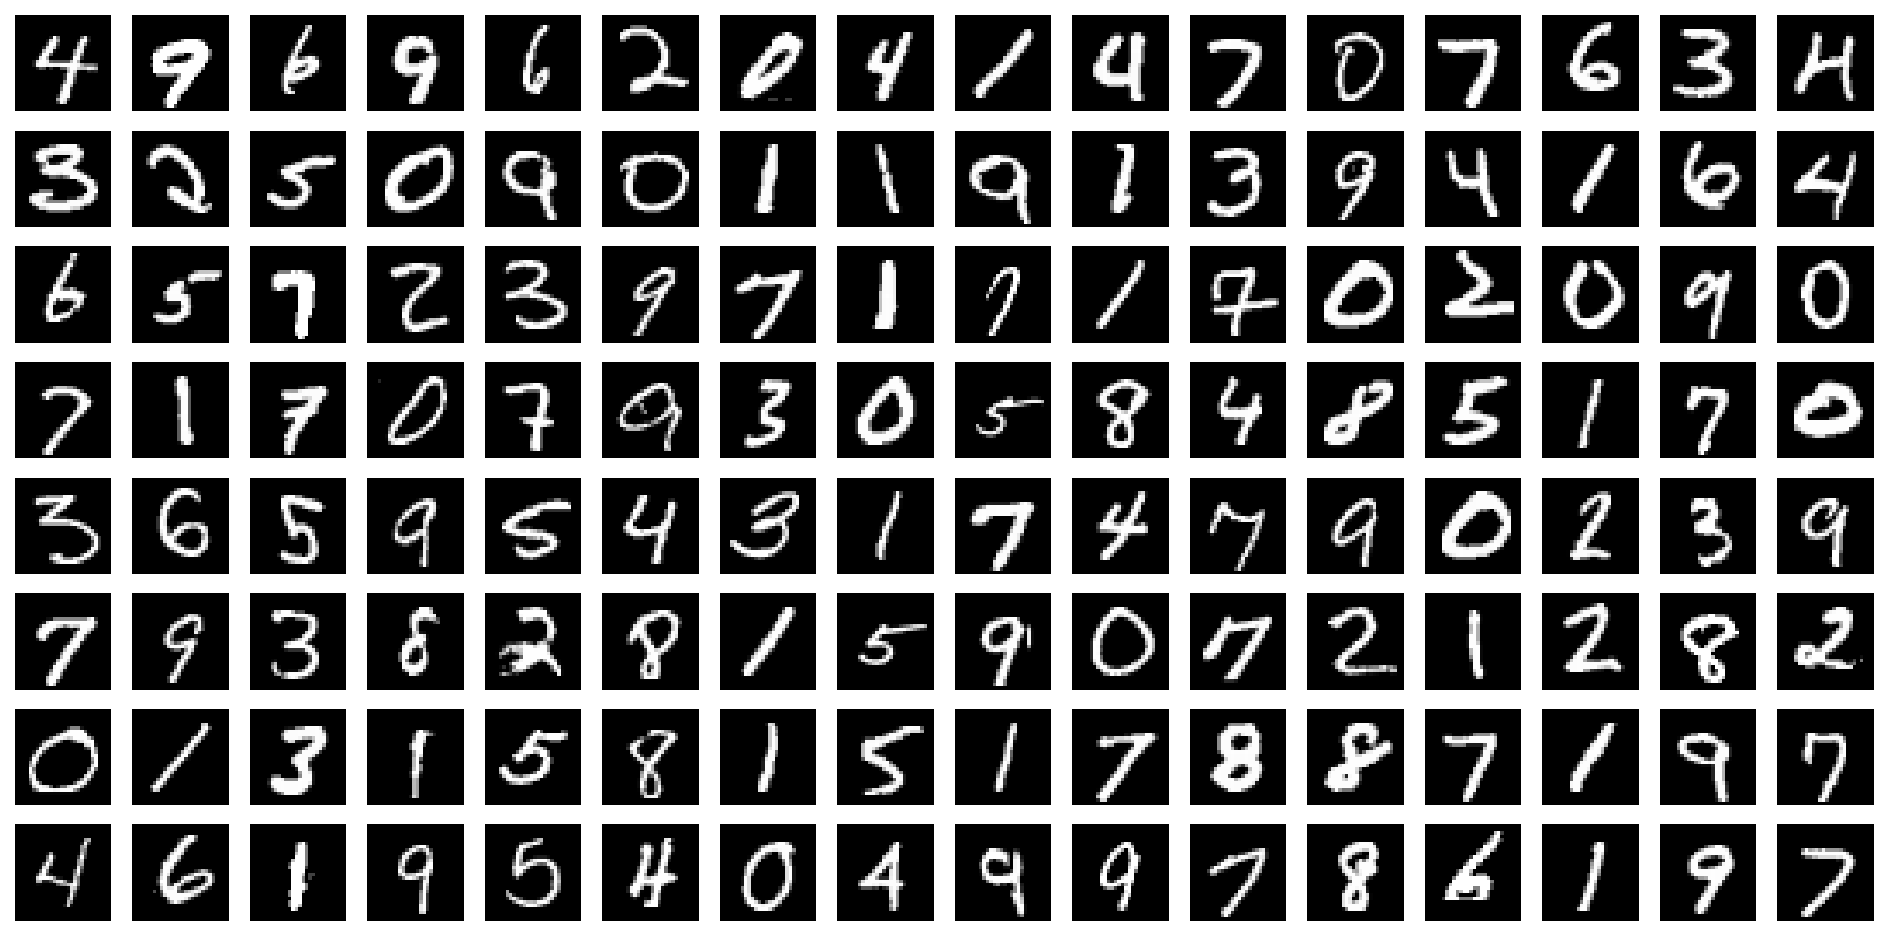
\includegraphics[width=\textwidth]{figures/mnist_random_grid_view.pdf}
\caption{MNIST数据集随机选取的$8\times 16$个样本构成的网格图}
\label{fig:mnist_random_grid_view}
\end{figure}

MNIST是非常经典的机器学习数据集,经常用作测试机器学习模型,特别是深度学习模型分类效果的基准数据集。尽管随着深度学习的发展,MNIST数据集由于规模偏小,已经不适用于评测计算机视觉领域的大模型,特别是近年来涌现的Vision Transformer\cite{dosovitskiy2021_vit},逐渐被ImageNet\cite{deng2009imagenet}, JFT-300M\cite{Sun_2017_JFT-300M}等大型数据集所取代,但经过合适处理\cite{mcmahan2017fed_avg, caldas2018_leaf, sahu2018fedprox}的MNIST数据集,作为联邦学习,特别是跨设备 (Cross-Silo) 场景的联邦学习的算法评测基准数据集,仍然是非常合适以及常用的\cite{reddi2020fed_opt, tran2021feddr, Ghosh_2022_cfl, li2021pfedmac, t2020pfedme}。

EMNIST数据集 (Extended MNIST database)\cite{cohen2017emnist} 是MNIST数据集的一个扩展,添加了手写的有大小写之分的26个英文字母图片,共计62类。EMNIST数据集也是常用的联邦学习的算法评测基准数据集\cite{sahu2018fedprox, zhang2020fedpd, acar2021feddyn}。数据集MNIST和EMNIST都来源于美国国家标准技术研究所 (National Institute of Standards and Technology, NIST)的手写表格和字符数据库 (Handprinted Forms and Characters Database)\cite{nist-19}。

联邦学习仿真系统\texttt{fl-sim}在\texttt{data\_processing}模块收录的MNIST/EMNIST相关的联邦数据集有
\begin{itemize}
    \item \texttt{FedMNIST}:(依照参考文献\parencite{sahu2018fedprox}的处理方式,并基于FedML\cite{he_2020_fedml}的实现) 将数据分为1000份 (1000个子节点),每份数据只有2类手写数字,每份数据的样本量的分布遵循幂律 (Power Law)。
    \item \texttt{FedEMNIST}:(依照参考文献\parencite[附录C.2]{reddi2020fed_opt}的处理方式,并基于FedML\cite{he_2020_fedml}的实现) 将数据集按书写者分为3400份 (3400个子节点)。
    \item \texttt{FedProxFEMNIST}:(依照参考文献\parencite{sahu2018fedprox}特殊处理过的EMNIST数据集的子集) 选取EMNIST数据集中的10类 (手写的小写英文字母``a''--``j'') 随机分为200份 (200个子节点),每一份数据只包含10个类别中的5类。
    \item \texttt{FedRotatedMNIST}:(依照参考文献\parencite{Ghosh_2022_cfl}特殊处理的MNIST数据集) 将每幅图片旋转多个角度 (例如$0^\circ, 90^\circ, 180^\circ, 270^\circ$),并将数据平均分配成多份 (多个子节点),保证每一份数据上图片旋转的角度一致 (例如都旋转了$90^\circ$)。这样一来,参与联邦学习训练的节点自然形成了多个聚落 (Cluster),非常适合用于评测聚类联邦学习相关的算法。
\end{itemize}

CIFAR10/100数据集\cite{cifar}由抓取自互联网并统一降采样为$32\times 32$像素大小的RGB~3通道图片组成,共有60000张图片,分为10/100类,以作者的工作单位加拿大高等研究所 (Canadian Institute for Advanced Research) 命名。图\ref{fig:cifar10_random_grid_view}~是从CIFAR10数据集中随机抽取$8\times 16$张图片组成的网格图。CIFAR10/100也是目前联邦学习理论及算法研究中最常用的基准数据集之一\cite{zhang2020fedpd, acar2021feddyn, Ghosh_2022_cfl}。

\begin{figure}[ht]
\centering
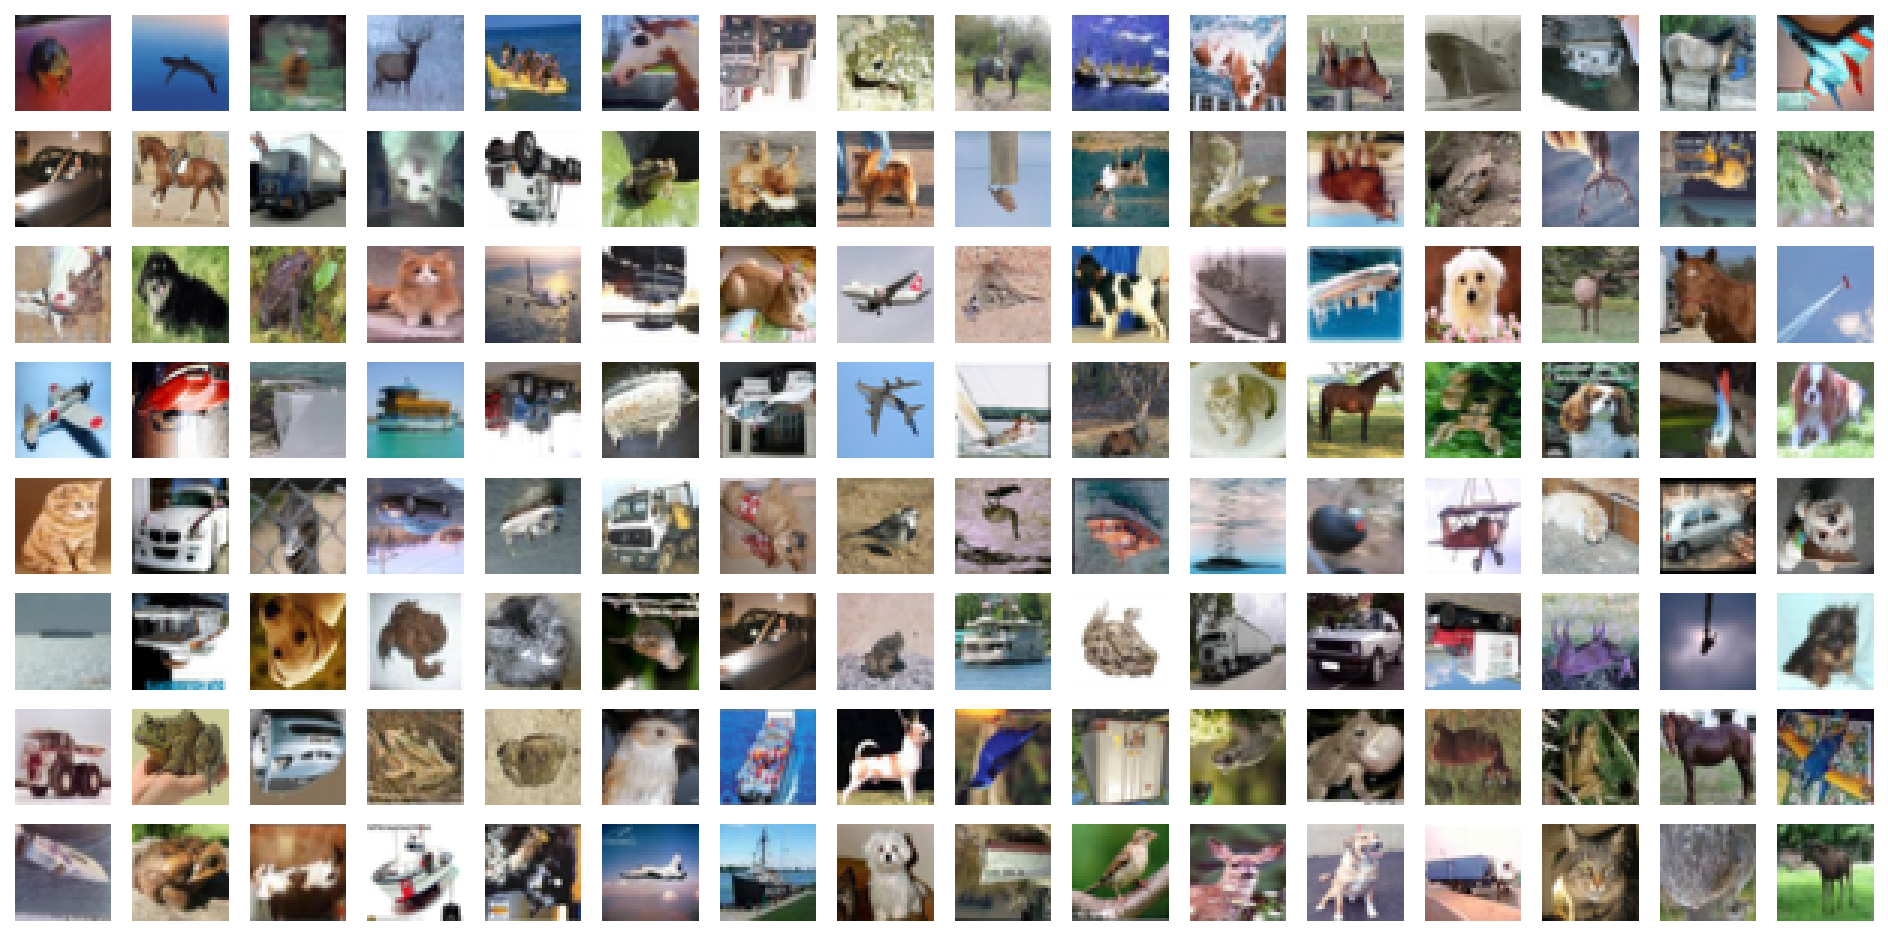
\includegraphics[width=\textwidth]{figures/cifar10_random_grid_view.pdf}
\caption{CIFAR10数据集随机选取的$8\times 16$个样本构成的网格图}
\label{fig:cifar10_random_grid_view}
\end{figure}

联邦学习仿真系统\texttt{fl-sim}在\texttt{data\_processing}模块收录的CIFAR10/100相关的联邦数据集有
\begin{itemize}
    \item \texttt{FedCIFAR100}:(依照TensorFlow Federated\footnote{\url{https://www.tensorflow.org/federated}}的处理方式,并基于FedML\cite{he_2020_fedml}的实现) 基于CIFAR100数据集的粗标签 (Coarse Label) 以及细标签 (Fine Label) 这一两层的标签结构,利用两层的隐狄利克雷分布 (Latent Dirichlet Allocation, LDA) \index{隐狄利克雷分布, Latent Dirichlet Allocation, LDA}\cite{Li_2006_LDA}将50000张训练集的图像均分为500份 (500个子节点)。类似地,10000张训练集的图像被平均分配到了前100个子节点上。值得注意的是,在这种分配方式下,并不是所有子节点上都有测试数据。
    \item \texttt{FedRotatedCIFAR10}:生成方式与\texttt{FedRotatedMNIST}\cite{Ghosh_2022_cfl}类似,不同之处在于基础数据集从MNIST替换为了CIFAR10。
\end{itemize}

以上是联邦学习仿真系统\texttt{fl-sim}集成的主要的一些计算机视觉相关的联邦数据集,相关的用于基准测试的任务是图像分类预测,损失函数为交叉熵损失。\texttt{fl-sim}为这些数据集预置了几个典型\cite{mcmahan2017fed_avg, zhang2020fedpd, sahu2018fedprox}的卷积神经网络模型以及多层感知机模型作为基准测试模型。

Shakespeare数据集是构建自莎士比亚全集 (The Complete Works of William Shakespeare,主要是戏剧)\footnote{\url{https://www.gutenberg.org/ebooks/100}} 的联邦学习数据集,首次提出是在参考文献\parencite{mcmahan2017fed_avg}中。随后联邦学习相关的软件库LEAF\cite{caldas2018_leaf}, TensorFlow Federated,以及FedML\cite{he_2020_fedml}等都对Shakespeare数据集进行了调整。联邦学习仿真系统\texttt{fl-sim}提供的相关联邦学习数据集\texttt{FedShakespeare}主要遵循了FedML\cite{he_2020_fedml}的处理方式,将Shakespeare数据集按戏剧作品的角色分为了715份 (715个子节点), 即每份数据都是同一个戏剧角色的台词。数据集\texttt{FedShakespeare}相关的机器学习任务一般是下一字符预测。联邦学习仿真系统\texttt{fl-sim}预置了一个循环神经网络模型\cite{mcmahan2017fed_avg}作为基准测试模型。

Sent140数据集\cite{sent140}是从社交网站推特 (Twitter) 爬取的数据集,其内容是推特用户发表的个人动态 (有字数限制),经过人工打标签,分为正面情绪、负面情绪两类。Sent140数据集由参考文献\parencite{sahu2018fedprox}首次引入联邦学习的研究领域。联邦学习仿真系统\texttt{fl-sim}提供的相关联邦数据集\texttt{FedProxSent140}遵循了参考文献\parencite{sahu2018fedprox}的处理方式:按用户将数据集Sent140分为772份 (772个子节点),即每份数据都是同一个用户在推特发表的个人动态。联邦数据集\texttt{FedProxSent140}预置的基准测试模型是一个循环神经网络模型\cite{sahu2018fedprox},做二分类的正、负面情感分类。

除了以上的计算机视觉以及自然语言处理相关的联邦数据集之外,联邦学习仿真系统\texttt{fl-sim}还集成了参考文献\parencite{sahu2018fedprox}提出的人造数据集 (Synthetic Dataset),命名为\texttt{FedSynthetic}。具体来说,子节点$k$上的数据$(x, y)$依照如下的关系 (一个简单的线性模型) 生成
\begin{equation}
\label{eq:fed-synthetic}
y = \argmax \left( \operatorname{softmax} \left( W_kx + b_k \right) \right),
\end{equation}
其中$x \in \R^{n}, W_k \in \R^{c \times n}, b_k \in \R^{c},$ $c$是可以设置的分类问题类别数目,$n$是是可以设置的特征维数。矩阵$W_k, b_k$的元素随机选取自均值为$u_k,$ 方差为$1$的正态分布:
\begin{equation*}
W_k \sim \mathcal{N}(u_k, 1), \quad b_k \sim \mathcal{N}(u_k, 1),
\end{equation*}
而$u_k$本身也随机选取自均值为$0,$ 方差为$\alpha \in \R$的正态分布:
\begin{equation*}
u_k \sim \mathcal{N}(0, \alpha).
\end{equation*}
自变量 (特征) $x$随机采样自均值为$v_k \in \R^n,$ 协方差矩阵为$\Sigma$的正态分布:
\begin{equation*}
x \sim \mathcal{N}(v_k, \Sigma),
\end{equation*}
其中协方差矩阵$\Sigma$为对角矩阵,且满足$\Sigma_{jj} = j^{-1.2},$ $j = 1, \ldots, n;$ 均值向量$v$的元素选取自均值为$B_k,$ 方差为$1$的正态分布
\begin{equation*}
v_k \sim \mathcal{N}(B_k, 1),
\end{equation*}
而$B_k$本身选取自均值为$0,$ 方差为$\beta \in \R$的正态分布:
\begin{equation*}
B_k \sim \mathcal{N}(0, \beta).
\end{equation*}
可以看到,若$\alpha$或者$\beta$取$0,$ 那么相应的$u_k$或者$B_k$只能取值为$0,$ 从而$W_k, b_k$或者$v_k$只能取与$k$无关的同一个正态分布,或是标准正态分布$\mathcal{N}(0, 1),$ 或是$\mathcal{N}(0, \Sigma).$ 可以说$\alpha$和$\beta$决定了联邦数据集\texttt{FedSynthetic}的统计异质性的特点。此联邦数据集预置的基准测试模型是多层感知机模型。
